%%%%%%%%%%%%%%%%%%%%%%%%%BORRAR
\documentclass[a4paper]{article}
\usepackage[utf8]{inputenc}
\usepackage[spanish, es-tabla]{babel}

\usepackage[a4paper, footnotesep = 1cm, width=18cm, left=2cm, top=2.5cm, height=25cm, textwidth=18cm, textheight=25cm]{geometry}
%\geometry{showframe}

\usepackage{tikz}
\usepackage{amsmath}
\usepackage{amsfonts}
\usepackage{amssymb}
\usepackage{float}
\usepackage{graphicx}
\usepackage{caption}
\usepackage{subcaption}
\usepackage{multicol}
\usepackage{multirow}
\setlength{\doublerulesep}{\arrayrulewidth}
\usepackage{xcolor}

\usepackage{hyperref}
\hypersetup{
    colorlinks=true,
    linkcolor=blue,
    filecolor=magenta,      
    urlcolor=blue,
    citecolor=blue,    
}

\newcommand{\quotes}[1]{``#1''}
\usepackage{array}
\newcolumntype{C}[1]{>{\centering\let\newline\\\arraybackslash\hspace{0pt}}m{#1}}
\usepackage[american]{circuitikz}
\usepackage{fancyhdr}
\usepackage{units} 

\pagestyle{fancy}
\fancyhf{}
\lhead{22.13 Electrónica III}
\rhead{Mechoulam, Lambertucci, Martorell, Londero}
\rfoot{\center \thepage}
\begin{document}
\section{auxiliar}
\tableofcontents
%%%%%%%%%%%%%%%%%%%%%%%%%BORRAR

\subsection{Introducción}
\subsubsection{Contadores}
		Los contadores son dispositivos digitales capaces de almacenar la cantidad de pulsos que este recibe. Como todo almacenamiento digital requiere de memoria, los contadores están generalmente constituidos por varias celdas de almacenamiento de 1 bit, comúnmente usados los JK flip-flops. Se puede contemplar la implementación de un JK flip-flop en la Figura (\ref{circ:fkflipflop}) utilizando solamente compuertas lógicas discretas. 
		
		\begin{figure}[H]
	\hspace*{-1cm}
	\centering
	\scalebox{0.7}{
	\begin{circuitikz}
		\draw	
	
			%%%%%%%%%%%%%%%%%%%%%%%%%%%%%
			%FIGURAS
			%%%%%%%%%%%%%%%%%%%%%%%%%%%%%
			
			node[nor port](nor1){} %NOR1
				to[open] ++ (0, -2)
			node[nor port](nor2){} %NOR2
			
			(nor1.in 1) to[open] ++ (-2, 0)
			node[and port, number inputs = 3](and1){} %AND1
			
			(nor2.in 2) to[open] ++ (-2, 0)
			node[and port, number inputs = 3](and2){} %AND2
			
			%%%%%%%%%%%%%%%%%%%%%%%%%%%%%	
	
			(nor1.out) to[short, -*] ++ (0.5, 0)
					node[](feedback1){}
				to[short] ++ (0.5, 0)
				to[short, -o] ++ (0.5, 0)
					node[](feedback2){}
				node[label=east:$Q$]{}
			
			(nor2.out) to[short, -*] ++ (0.5, 0)
					node[](feedback3){}
				to[short] ++ (0.5, 0)
					node[](feedback4){}
				to[short,-o] ++ (0.5, 0)
				node[label=east:$\overline{Q}$]{}
				
			(feedback1) to[short] ++ (0, -0.38)
				to[short] ++ (-3, -1)
				to[short] ++ (0, -0.3)
				|- (nor2.in 1)
				
			(feedback3) to[short] ++ (0, 0.38)
				to[short] ++ (-3, 1)
				to[short] ++ (0, 0.3)
				|- (nor1.in 2)
				
			(nor1.in 1) -- (and1.out)
			(nor2.in 2) -- (and2.out)
			
			(and1.in 2) to[short, -o] ++ (-1, 0)
				node[label=west:$J$]{}
			
			(and2.in 2) to[short, -o] ++ (-1, 0)
				node[label=west:$K$]{}
				
			(and1.in 3) to[short] ++ (-0.5, 0)
				to[short, -*] ++ (0, -0.922)
				node[](enable){}
				|- (and2.in 1)
				
			(and2.in 3)	to[short] ++ (-0.5, 0)
				|- ++ (5.5, -0.5)
				-| (feedback3.center)
				
			(and1.in 1) to[short] ++ (-0.5, 0)
				|- ++ (5.5, 0.6)
				-| (feedback1.center)
				
			(enable) to[short] ++ (-0.5, 0)
				to[twoport, -o, l_=Edge Det] ++ (-3, 0)
				node[label=west:$CLK$]{}
	
		;
	\end{circuitikz}
	}
	\caption{Implementación de un JK flip-flop con una totalidad de 8 compuertas lógicas discretas (teniendo en cuenta la implementación de las compuertas AND de tres entradas junto a la corrección de delay.}
	\label{circ:fkflipflop}
\end{figure}
		
		La cantidad de flip-flops necesaria para construir un contador está ligada al mayor número que el dispositivo puede almacenar. Si se quiere contar hasta el número $N$, el contador tendrá que disponer como mínimo de $\lceil log_2(N) \rceil$ flip-flops. Existen dos tipos de contadores: asíncronos y síncronos.
		
\subsubsection{Contadores Asíncronos}
		Los contadores asíncronos poseen un único flip-flop cuya entrada esté conectada al generador de pulsos, propagándose la información provista por este a través del resto para aumentar el contador. Es por esta razón que a los contadores asíncronos se los suele denominar también como contadores por propagación o \textit{ripple counters} en inglés. 

\begin{figure}[H]
	\centering
	\begin{circuitikz}
		\draw
			node[ocirc, label=west:$CLK$]{}
				to[short] ++ (1, 0)
				to[open] ++ (2, 1)
				node[fourport](1){}
				to[open] ++ (3, 0)
				node[fourport](2){}
				to[open] ++ (3, 0)
				node[fourport](3){}
				to[open] ++ (3, 0)
				node[fourport](4){}
				to[open] ++ (-11, -1)
				|- (1.1)
				(1.2) -- (2.1)
				(2.2) -- (3.1)
				(3.2) -- (4.1)
				
				(1.1) ++ (0.13,0) node[]{\scalebox{1.2}{\rotatebox{-90}{$\triangle$}}}
				(2.1) ++ (0.13,0) node[]{\scalebox{1.2}{\rotatebox{-90}{$\triangle$}}}
				(3.1) ++ (0.13,0) node[]{\scalebox{1.2}{\rotatebox{-90}{$\triangle$}}}
				(4.1) ++ (0.13,0) node[]{\scalebox{1.2}{\rotatebox{-90}{$\triangle$}}}
		;
	\end{circuitikz}
	\caption{Conección entre flip-flops para un contador asíncrono.}
	\label{circ:async_counter_connection}		
\end{figure}				
		
	Como los pulsos deben de propagarse a lo largo de varias compuertas lógicas, sucede que para cada incremento en el contador, no todos los bits de la palabra almacenada cambian al mismo instante. En la Figura (\ref{async_ripple}) se esquematiza este efecto para un contador que transita de almacenar un $0111_2$ a almacenar un $1000_2$.

\begin{figure}[H]
	\centering
	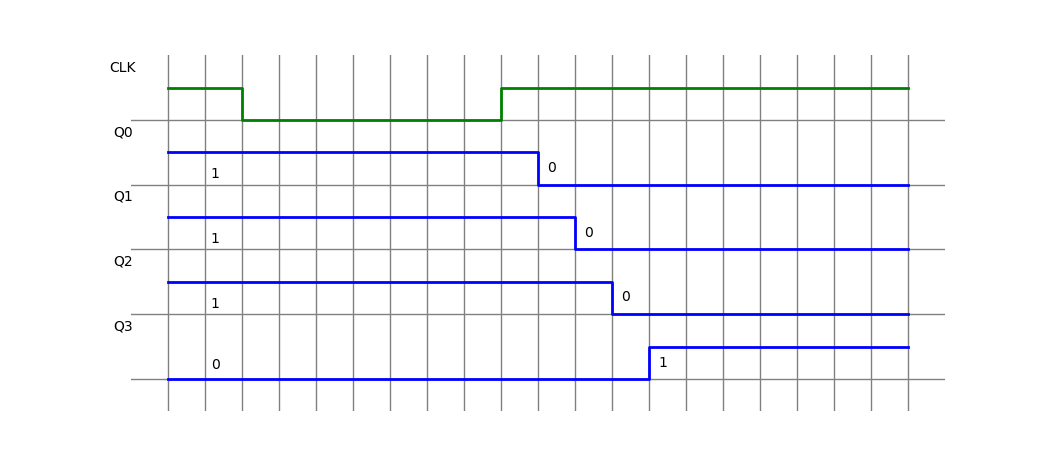
\includegraphics[width=0.7\textwidth]{Imagenes/async_ripple.png}
	\caption{Propagación de un pulso recibido a través de un contador asíncrono para la palabra almacenada transitando del estado $(7)_{10}$ al estado $(8)_{10}$.}
	\label{async_ripple}
\end{figure}

	Debido a este fenómeno, las implementaciones asíncronas de contadores no son del todo fidedignas. Sin embargo, abundan como divisores de frecuencia ya que la salida de cada flip-flop será la frecuencia de los pulsos de entrada dividida por una potencia de dos. Otra desventaja de los contadores asíncronos está directamente relacionada con la anterior y es que debido al fenómeno de propagación estos dispositivos se vuelven mucho más lentos en comparación a otros tipos de contadores. No obstante, la ventaja de esta implementación es que estos dispositivos son muy simples y fáciles de contruir.

\subsubsection{Contadores Síncronos}

Los contadores síncronos poseen todos sus flip-flops conectados al generador de pulsos. Por esta razón, se elimina la propagación presente en los contadores asíncronos y los problemas que este fenómeno deriva.

\begin{figure}[H]
	\centering
	\begin{circuitikz}
		\draw
			node[ocirc, label=west:$CLK$]{}
				to[short] ++ (1, 0)
					node[](hola){}
				to[open] ++ (2, 1.5)
				node[fourport](1){}
				to[open] ++ (3, 0)
				node[fourport](2){}
				to[open] ++ (3, 0)
				node[fourport](3){}
				to[open] ++ (3, 0)
				node[fourport](4){}
				to[open] ++ (-11, -1)

				(1.1) to[short] ++ (-0.5,0)
					to[short, -*] ++ (0, -1.05)
				(2.1) to[short] ++ (-0.5,0)
					to[short, -*] ++ (0, -1.05)
				(3.1) to[short] ++ (-0.5,0)
					to[short, -*] ++ (0, -1.05)
				(4.1) to[short] ++ (-0.5,0)
					to[short] ++ (0, -1.05)
					to[short] (hola)
				
				
				
				(1.1) ++ (0.13,0) node[]{\scalebox{1.2}{\rotatebox{-90}{$\triangle$}}}
				(2.1) ++ (0.13,0) node[]{\scalebox{1.2}{\rotatebox{-90}{$\triangle$}}}
				(3.1) ++ (0.13,0) node[]{\scalebox{1.2}{\rotatebox{-90}{$\triangle$}}}
				(4.1) ++ (0.13,0) node[]{\scalebox{1.2}{\rotatebox{-90}{$\triangle$}}}
		;
	\end{circuitikz}
	\caption{Conección entre flip-flops para un contador síncrono.}
	\label{circ:sync_counter_connection}		
\end{figure}

Es por esta razón que no solo los contadores síncronos son una implementación segura para contar, sino que también son más rápidos que su contraparte asíncrona. No obstante, la complejidad de estos dispositivos aumenta considerablemente.

\subsection{Implementaciones y Mediciones}
\subsubsection{Contador Asíncrono}
En la Figura (\ref{fig:async_circ}) se puede observar la implementación realizada en PCB.

\begin{figure}[H]
	\centering
	\begin{circuitikz}
		\draw
			%%%%%%%%%%%%%%%%%%%%%%%%%%%%%%
			%Figuras
			%%%%%%%%%%%%%%%%%%%%%%%%%%%%%%
			(-3,-2)
			node[ocirc, label=west:$CLK$](CLK){}	
			
			(0,0)
			node[fourport](FF1){}
				(FF1.1) ++ (0.12,0.43) node[]{\scalebox{1.2}{\rotatebox{-90}{$\triangle$}}}
				 ++ (-0.12,0) node[](FF1_CLK){}
				(FF1.1) ++ (0.15, -0.12) node[](){$K$}
					node[](FF1_1){}
				(FF1.2) ++ (-0.15, -0.12) node[](){$\overline{Q}$}
				node[](FF1_2){}
				(FF1.3) ++ (-0.15, 0.12) node[](){$Q$}
				node[](FF1_3){}
				(FF1.4) ++ (0.15, 0.12) node[](){$J$}
				node[](FF1_4){}
				(FF1_CLK) to[short] ++ (-0.5, 0)
					node[](FF1_CLK){}
				(FF1.1) to[short] ++ (-0.5, 0)
					node[](FF1_1){}
				(FF1.2) to[short] ++ (0.5, 0)
					node[](FF1_2){}
				(FF1.3) to[short] ++ (0.5, 0)
					node[](FF1_3){}
					to[short, -o] ++ (0, 2)
					node[label=north:$Q_0$]{}
				(FF1.4) to[short] ++ (-0.5, 0)
					node[](FF1_4){}
			
			(4,0)
			node[fourport](FF2){}
				(FF2.1) ++ (0.12,0.43) node[]{\scalebox{1.2}{\rotatebox{-90}{$\triangle$}}}
				++ (-0.12, 0) node[](FF2_CLK){}
				(FF2.1) ++ (0.15, -0.12) node[](){$K$}
				(FF2.2) ++ (-0.15, -0.12) node[](){$\overline{Q}$}
				(FF2.3) ++ (-0.15, 0.12) node[](){$Q$}
				(FF2.4) ++ (0.15, 0.12) node[](){$J$}
				(FF2_CLK) to[short] ++ (-0.5, 0)
					node[](FF2_CLK){}
				(FF2.1) to[short] ++ (-0.5, 0)
					node[](FF2_1){}
				(FF2.2) to[short] ++ (0.5, 0)
					node[](FF2_2){}
				(FF2.3) to[short] ++ (0.5, 0)
					node[](FF2_3){}
					to[short, -o] ++ (0, 2)
					node[label=north:$Q_1$]{}
				(FF2.4) to[short] ++ (-0.5, 0)
					node[](FF2_4){}
			
			(8,0)
			node[fourport](FF3){}
				(FF3.1) ++ (0.12,0.43) node[]{\scalebox{1.2}{\rotatebox{-90}{$\triangle$}}}
				++ (-0.12, 0) node[](FF3_CLK){}
				(FF3.1) ++ (0.15, -0.12) node[](){$K$}
				(FF3.2) ++ (-0.15, -0.12) node[](){$\overline{Q}$}
				(FF3.3) ++ (-0.15, 0.12) node[](){$Q$}
				(FF3.4) ++ (0.15, 0.12) node[](){$J$}
				(FF3_CLK) to[short] ++ (-0.5, 0)
					node[](FF3_CLK){}
				(FF3.1) to[short] ++ (-0.5, 0)
					node[](FF3_1){}
				(FF3.2) to[short] ++ (0.5, 0)
					node[plain crossing, rotate=45](FF3_2){}
				(FF3.3) to[short] ++ (0.5, 0)
					node[](FF3_3){}
					to[short, -o] ++ (0, 2)
					node[label=north:$Q_2$]{}
				(FF3.4) to[short] ++ (-0.5, 0)
					node[](FF3_4){}
			%%%%%%%%%%%%%%%%%%%%%%%%%%%%%%
			%FF1, FF2, FF3, CLK
			%%%%%%%%%%%%%%%%%%%%%%%%%%%%%%
			(CLK) to[short] ++ (1, 0) |- (FF1_CLK.center)
				
			(FF1_1) to[short, -*] (FF1_4)
			(FF2_1) to[short, -*] (FF2_4)
			(FF3_1) to[short, -*] (FF3_4)
			
			(FF1_4) to[short, -*] ++ (0, 1)
			(FF2_4) to[short, -*] ++ (0, 1)
			(FF3_4) to[short] ++ (0, 1)
				to[short] ++ (-9.5, 0)
				node[ocirc, label=west:$1$](){}
			%(spdt.out 1) to[short, -o] ++ (-0.5, 0)
			%	node[label=west:$1$]{}
			%(spdt.out 2) to[short, -o] ++ (-0.5, 0)
			%	node[label=west:$0$]{}
			
			(FF3_CLK) to[open] ++ (-0.6, 0)
				node[spdt, rotate=180, yscale=-1](sw1){}
				
			(FF2_CLK) to[open] ++ (-0.6, 0)
				node[spdt, rotate=180, yscale=-1](sw2){}
				
			(sw1.out 1) to[short, -*] ++ (0, 0.15)
			(sw2.out 1) to[short, -*] ++ (0, 0.15)
			(sw1.out 2) to[short] ++ (0, -0.11)
			(sw2.out 2) to[short] ++ (0, -0.11)
		;
	\end{circuitikz}
	\caption{Implementación de contador asíncrono.}
	\label{fig:async_circ}
\end{figure}

\subsubsection{Contador Síncrono}
En la Figura (\ref{fig:sync_circ}) se puede observar la implementación realizada en PCB.

\begin{figure}[H]
	\centering
	\begin{circuitikz}
		\draw
			%%%%%%%%%%%%%%%%%%%%%%%%%%%%%%
			%Figuras
			%%%%%%%%%%%%%%%%%%%%%%%%%%%%%%
			(-3,-2)
			node[ocirc, label=west:$CLK$](CLK){}	
			
			(0,0)
			node[fourport](FF1){}
				(FF1.1) ++ (0.12,0.43) node[]{\scalebox{1.2}{\rotatebox{-90}{$\triangle$}}}
				 ++ (-0.12,0) node[](FF1_CLK){}
				(FF1.1) ++ (0.15, -0.12) node[](){$K$}
					node[](FF1_1){}
				(FF1.2) ++ (-0.15, -0.12) node[](){$\overline{Q}$}
				node[](FF1_2){}
				(FF1.3) ++ (-0.15, 0.12) node[](){$Q$}
				node[](FF1_3){}
				(FF1.4) ++ (0.15, 0.12) node[](){$J$}
				node[](FF1_4){}
				(FF1_CLK) to[short] ++ (-0.5, 0)
					node[](FF1_CLK){}
				(FF1.1) to[short] ++ (-0.5, 0)
					node[](FF1_1){}
				(FF1.2) to[short] ++ (0.5, 0)
					node[](FF1_2){}
				(FF1.3) to[short] ++ (0.5, 0)
					node[](FF1_3){}
					to[short, -o] ++ (0, 2)
					node[label=north:$Q_0$]{}
				(FF1.4) to[short] ++ (-0.5, 0)
					node[circ](FF1_4){}
			
			(4,0)
			node[fourport](FF2){}
				(FF2.1) ++ (0.12,0.43) node[]{\scalebox{1.2}{\rotatebox{-90}{$\triangle$}}}
				++ (-0.12, 0) node[](FF2_CLK){}
				(FF2.1) ++ (0.15, -0.12) node[](){$K$}
				(FF2.2) ++ (-0.15, -0.12) node[](){$\overline{Q}$}
				(FF2.3) ++ (-0.15, 0.12) node[](){$Q$}
				(FF2.4) ++ (0.15, 0.12) node[](){$J$}
				(FF2_CLK) to[short] ++ (-0.5, 0)
					node[](FF2_CLK){}
				(FF2.1) to[short] ++ (-0.5, 0)
					node[](FF2_1){}
				(FF2.2) to[short] ++ (0.5, 0)
					node[](FF2_2){}
				(FF2.3) to[short] ++ (0.5, 0)
					node[](FF2_3){}
					to[short, -o] ++ (0, 2)
					node[label=north:$Q_1$]{}
				(FF2.4) to[short] ++ (-0.5, 0)
					node[circ](FF2_4){}
			
			(10,0)
			node[fourport](FF3){}
				(FF3.1) ++ (0.12,0.43) node[]{\scalebox{1.2}{\rotatebox{-90}{$\triangle$}}}
				++ (-0.12, 0) node[](FF3_CLK){}
				(FF3.1) ++ (0.15, -0.12) node[](){$K$}
				(FF3.2) ++ (-0.15, -0.12) node[](){$\overline{Q}$}
				(FF3.3) ++ (-0.15, 0.12) node[](){$Q$}
				(FF3.4) ++ (0.15, 0.12) node[](){$J$}
				(FF3_CLK) to[short] ++ (-0.5, 0)
					node[](FF3_CLK){}
				(FF3.1) to[short] ++ (-0.5, 0)
					node[](FF3_1){}
				(FF3.2) to[short] ++ (0.5, 0)
					node[plain crossing, rotate=45](FF3_2){}
				(FF3.3) to[short] ++ (0.5, 0)
					node[](FF3_3){}
					to[short, -o] ++ (0, 2)
					node[label=north:$Q_2$]{}
				(FF3.4) to[short] ++ (-0.5, 0)
					node[circ](FF3_4){}
			%%%%%%%%%%%%%%%%%%%%%%%%%%%%%%
			%FF1, FF2, FF3, CLK
			%%%%%%%%%%%%%%%%%%%%%%%%%%%%%%
			(CLK) to[short, -*] ++ (1, 0) |- (FF1_CLK.center)
			(CLK) to[open] ++ (1, 0) 
				to[short, -*] ++ (4, 0) |- (FF2_CLK.center)
			(CLK) to[open] ++ (5, 0)
				to[short] ++ (6, 0) |- (FF3_CLK.center)
				
			(FF1_1) to[short] (FF1_4)
			(FF2_1) to[short] (FF2_4)
			(FF3_1) to[short] (FF3_4)
			
			(FF1_4) to[short] ++ (0, 1)
				to[short] ++ (-1.5, 0)
				node[ocirc, label=west:$1$](){}
			
			
			(FF3_4) to[open] ++ (-2, 0)
			 	to[open] ++ (-0.6, 0)
				node[spdt, rotate=180, yscale=-1](sw1){}
			(sw1.out 1) node[circ]{}
			
			(FF3_4) ++ (-0.5, 0) node[and port, scale=0.7](and){}
				(FF3_4) to[short] ++ (-0.5,0)				
			
			(FF2_4) to[open] ++ (-0.6, 0)
				node[spdt, rotate=180, yscale=-1](sw2){}
			(sw2.out 1) node[circ]{}
			
			(FF1_2) to[short] (sw2.out 2)
			(FF2_2) to[short] (sw1.out 2)
			
			(sw1.in) |- (and.in 2)
			
			(FF2_4) to[short]++(0, 0.75)
				-| (and.in 1)
			
		;
	\end{circuitikz}
	\caption{Implementación de contador síncrono.}
	\label{fig:sync_circ}
\end{figure}

\subsubsection{Máxima Velocidad de Operación}

Se midió en una primera instancia el tiempo de propagación al realizar la acción de \textit{toggle} de un solo JK flip-flop, obteniéndose un valor de $191.21 ns$ para el establecimiento de $Q$ al valor previo de $\overline{Q}$. Luego, se midió la cantidad de tiempo entre un flanco ascendente de la señal de clock proporcionada al contador asíncrono y sincrónico, y el cambio del bit $Q_2$ de ambos contadores para el caso presentado en la Figura (\ref{async_ripple}). Los tiempos obtenidos fueron de $223.51 ns$ para el contador sincrónico y $738.32 ns$ para el contador asíncrono, poniendo en evidencia no sólo lo mucho más lento que es el contador asíncrono sino cuánto más rápido es un JK flip-flop integrado a uno implementado con compuertas lógicas discretas, ya que los integrados poseen un tiempo de propagación típico menor a $10ns$. 

\end{document}